\section{Early work at stable beam facilities}

\subsection{Caltech separator}

With the availability of heavy ion beams at energies which would allow radiative capture measurements in inverse kinematics, windowless gas targets were developed, which in several experiments showed an improved $\gamma$ detection environment due to a reduction in beam induced backgrounds. However, as nuclear astrophysics experiments usually need to push the boundary of the possible to reach the astrophysically relevant energy regimes (associated with low experimental yields), it was quickly realized that the small recoil cone angle associated with the emission of a radiative capture $\gamma$-ray would allow efficient reaction recoil detection for further background suppression through a coincidence requirement. The concept was first realized at the California Institute of Technology (Caltech) in the middle of the 1980's. The Caltech set-up used a heavy ion beam from the 3 MV Pelletron Tandem Accelerator at the Kellogg Radiation Laboratory. It consisted of a windowless, differentially pumped (two sided) gas target and a recoil separator using two separation stages, Fig. \ref{fig:caltech}.
\begin{figure}
\centering
\resizebox{0.6\columnwidth}{!}{
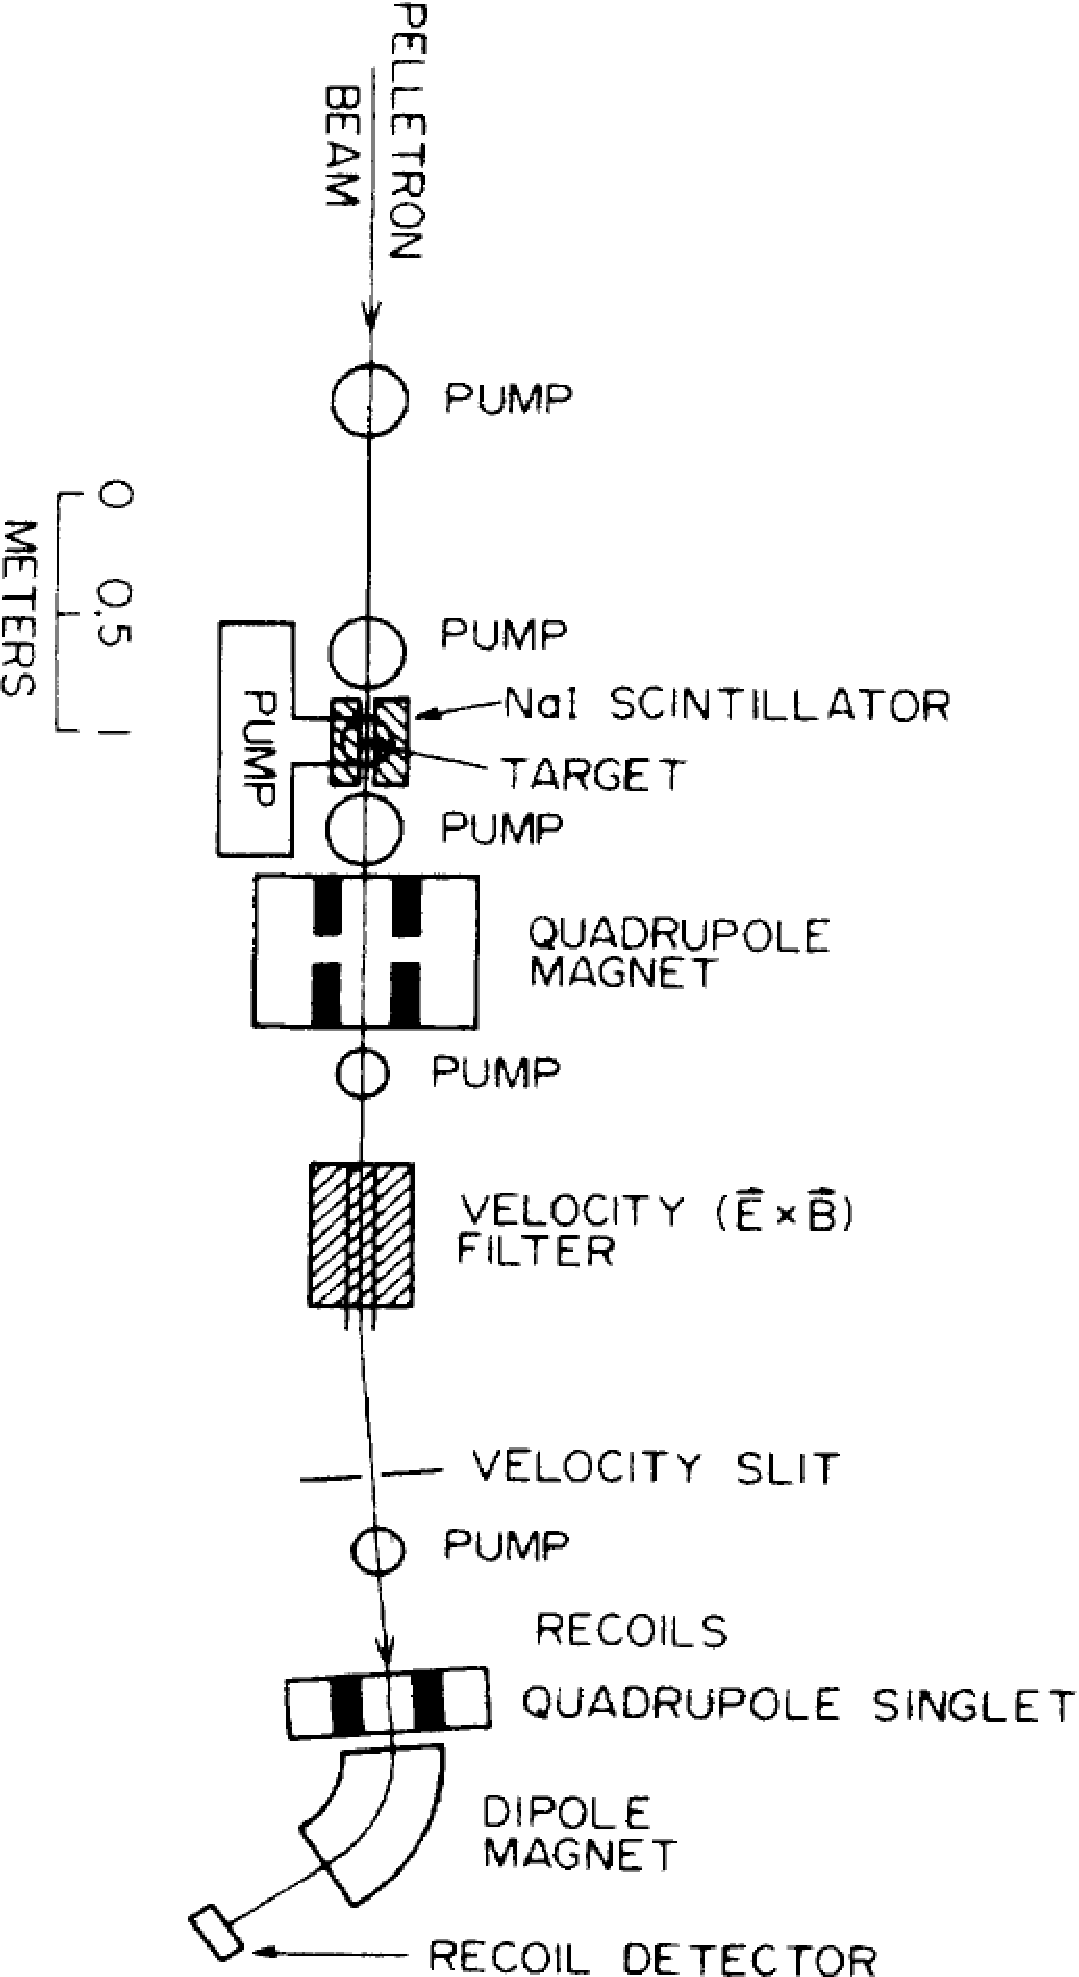
\includegraphics{Hahn87_Fig2_CaltechSeparator}
}
%\vspace{5cm}       % Give the correct figure height in cm
\caption{Schematic view of the Caltech separator. Taken from \cite{hahn87}.}
\label{fig:caltech}       % Give a unique label
\end{figure}
Immediately after emerging from the last pumping stage of the gas target (through conical gas flow limiters), the recoil cone was re-focussed by a quadrupole doublet onto a variable slit. Velocity filtering employing this slit was provided by a crossed field (Wien-) filter. Such an element transmits all charge states of a given velocity, and further cleanup of the recoils to the focal plane is provided by a dipole magnet through momentum and charge state selection. The transmitted recoils and “leaky” beam particles were detected with a two segment ionization chamber (IC) using $Z$-identification through the difference in energy loss. Additionally, a parallel grid proportional counter (PGAC) preceded the IC in a separate gas volume to provided a timing signal. The arrival of a particle at the end of the recoil separator provided the logical condition for an array of four large NaI detectors to allow recording of a possible gamma signal with over 50\% efficiency.\\ 
The Caltech separator was built for for the measurement of those alpha radiative capture reactions most relevant to stellar helium burning. In the important energy regime, cross sections of below $1 \unit{nb}$ and recoil cones above 15 mrad were expected. The setup was used for two published experiments: the design benchmark \nuc{12}{C}\reac{\alpha}{\gamma}\nuc{16}{O} \cite{krem88} and a determination of the direct capture component of \nuc{16}{O}\reac{\alpha}{\gamma}\nuc{20}{Ne} \cite{hahn87}. In both experiments, the recoil separator provided a beam suppression of the order of $10^8$ to $10^9$. The maximum count rate permissible in the focal plane detectors ($\approx 30 \unit{kHz}$) limited the beam current to be employed to a few micro-Ampere. At these high count rates a reliable reaction detection through evaluation of only the recoils in the focal plane was not attempted, instead the recoil detection was used as a trigger for the NaI gamma detector array. Although the available publications state no precise maximum acceptance numbers for the Caltech separator experiments, they reveal that for the \nuc{12}{C}\reac{\alpha}{\gamma}\nuc{16}{O} reaction only part of the reaction recoils could be transmitted, while the \nuc{16}{O}\reac{\alpha}{\gamma}\nuc{20}{Ne} reaction ($\frac{\Delta{}v}{v} \approx 2 \%$) recoil cone (due to the smaller $Q$-value) fit comfortably. Ray-trace simulation allowed to extract cross sections down to the $0.2 \unit{nb}$ range to be extracted from the experiments.\\ 
These pioneering measurements revealed clearly both the advantages and disadvantages of the recoil detection approach. The use of the recoil separator allowed the recording of background free gamma spectra. However, the available beam suppression factor limited the amount of beam current usable to the count rate capabilities of the focal plane detection system. Additionally, the dependence of recoil transmission on the $\gamma$-ray energy and emission angle, in this case of limited recoil cone acceptance, does not allow truly independent measurements. In the time period of the above cited measurements, discussions started about the realization of radioactive ion beam facilities. In the area of nuclear astrophysics radioactive ion beam measurements to elucidate the hot CNO cycle were perceived to be a primary aim. It was quickly realized that for the necessary proton radiative capture experiments the recoil separator approach would be ideal. In order to explore the usefulness of the existing Caltech setup for these types of projected experiments Smith {\it et al.} \cite{smit91} performed a series of measurements of the \nuc{12}{C}\reac{p}{\gamma}\nuc{13}{N} reaction focussing on direct \nuc{13}{N} recoil detection. Comparison of direct $\gamma$ capture yield, \nuc{13}{N} capture/activity determination, and \nuc{13}{N} direct recoil detection methods produced reliable results within errors proving the feasibility of the recoil separator approach. The collaborators on this experiment suggested the use of additional filter elements and/or baffles to improve the performance of future dedicated recoil separators at radioactive ion beam facilities. Additionally, they called for work on the improvement of focal plane detectors to allow better recoil identification.


\subsection{NABONA}

The first experiment attempting to measure radiative proton capture on a radioactive nucleus using a recoil separator was performed at a stable ion beam facility. In this case, like in many of the early nuclear astrophysics recoil separator setups, a set of existing beam line components (here from an accelerator mass spectrometry experiment) was adapted for the measurements. The goal of this effort was to determine the absolute cross section of radiative proton capture on \nuc{7}{Be}, which is a crucial reaction for predicting the neutrino spectrum emanating from our sun. In order to be competitive with previous efforts using a solid \nuc{7}{Be} target (which were possible due to the relatively long half-life of 52.9 days) the setup was designed to keep systematical errors at the 5\% level. This condition influenced the design of the windowless gas target, which, at a length of about 15 cm, was a factor three longer than the Caltech setup (and allowed for twice the gas cell pressure). However, the low $Q$-value of the \nuc{7}{Be}\reac{p}{\gamma}\nuc{8}{B} reaction results in a much smaller recoil cone than the alpha captures targeted at Caltech. At the NApoli-BOchum-Nuclear Astrophysics (NABONA) setup the acceptance was clearly available to provide full transmission for a selected recoil charge state. The Universita Federico II in Napoli, Italy, operates a 3 MV tandem accelerator, equipped with a sputter ion source, which was supplied with a \nuc{7}{Be} (produced at the ATOMKI, Hungary) sputter cathode. After momentum and charge analysis (selecting the $4^+$ charge state to suppress \nuc{7}{Li} beam components) the \nuc{7}{Be} beam was guided through the windowless gas target. In the NABONA approach, a dipole magnet was used first to select one charge state of both beam and recoils on a focus (achieved by a quadrupole doublet) through a pair of slits, see Fig. \ref{fig:nabona}.
\begin{figure}
\resizebox{0.9\columnwidth}{!}{
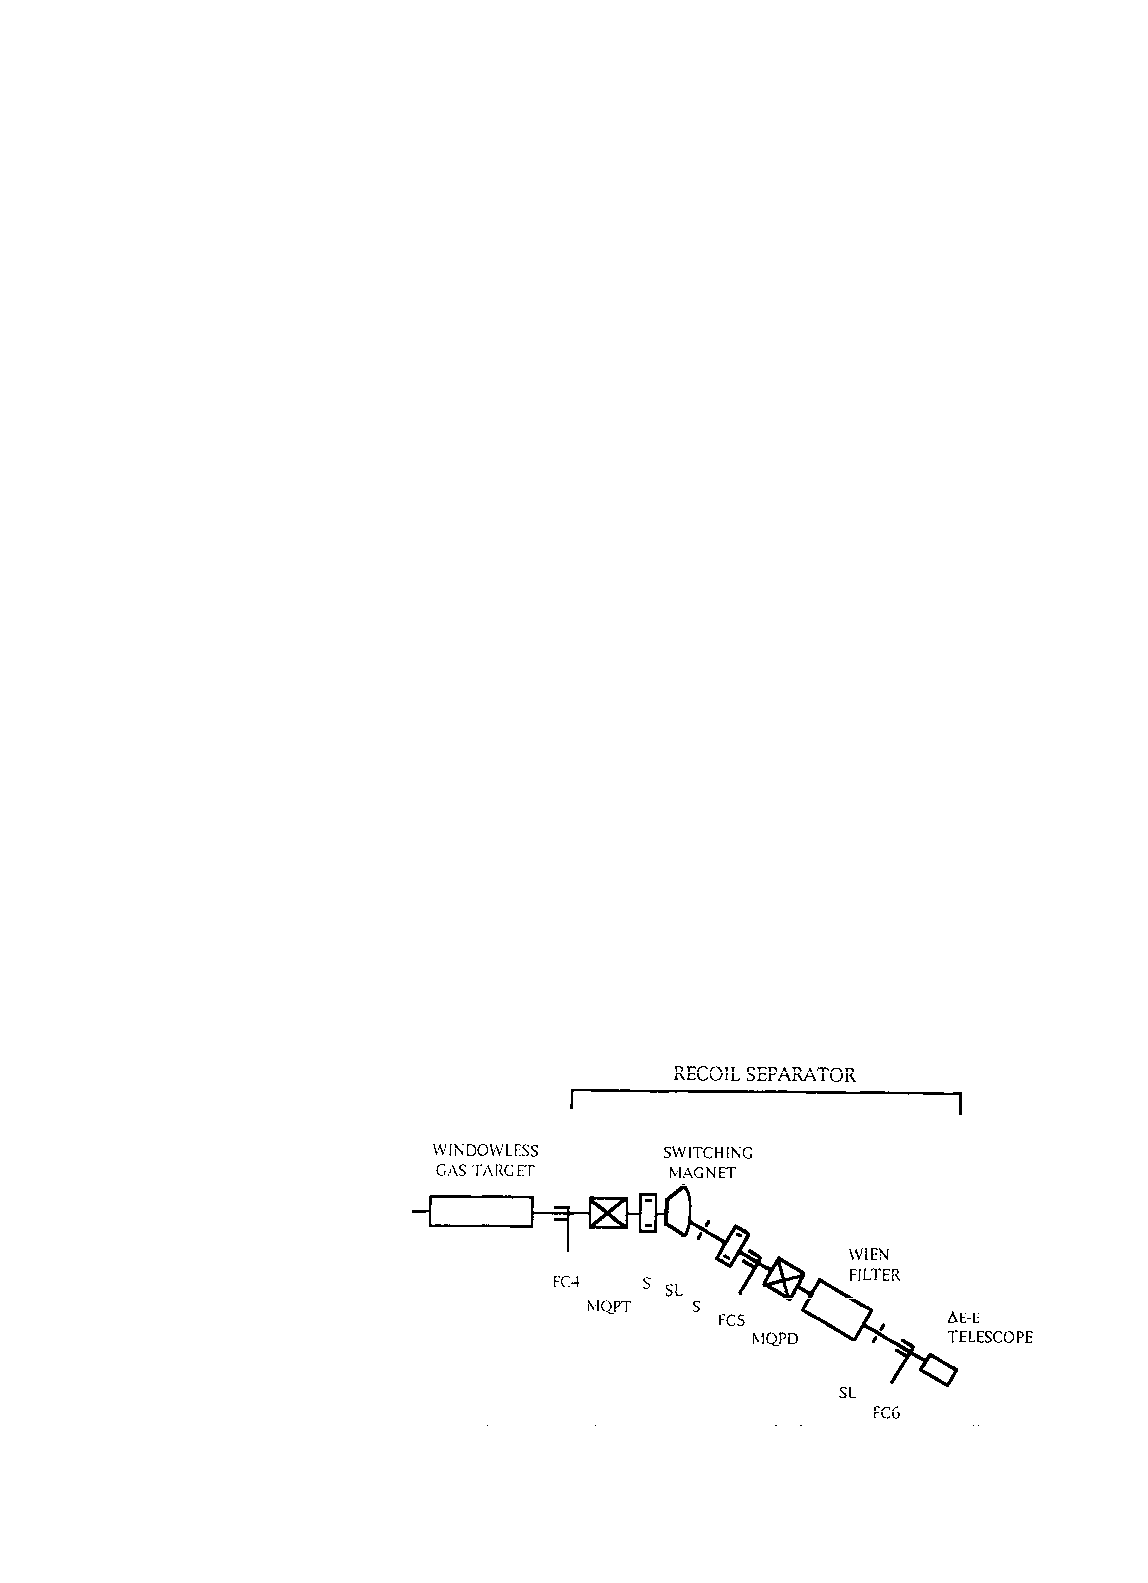
\includegraphics{Gialanella96_Fig1_NABONA}
}
%\vspace{5cm}       % Give the correct figure height in cm
\caption{Schematic view of the NABONA separator. Taken from \cite{gial96}.}
\label{fig:nabona}
\end{figure}
After traversing the charge selecting slits, another quadrupole focussed the ions towards the final focal plane. On the way, they passed a crossed field (Wien-) velocity filter, which was set to allow passage only for reaction recoils (beam and recoils have the same momentum, but differ in velocity). At the end of the separator, a two section $\Delta{}E$-$E$ ionization chamber provided recoil identification. The complete setup was tested carefully \cite{gial96}, using again the \nuc{12}{C}\reac{p}{\gamma}\nuc{13}{N} reaction to establish that the momentum distribution (also causing the recoil cone) of the \nuc{7}{Be}\reac{p}{\gamma}\nuc{8}{B} target reaction would fit into its acceptance. The observed value for $\frac{\Delta{}p}{p}$ amounted to $\approx1.9\%$ at slit settings which provided an incident \nuc{12}{C} beam suppression of $2\cdot10^{-10}$. The choice of gas flow limiting apertures allowed acceptance of recoils emerging within a cone of half-angle $0.4^\circ$. The resulting cross section measured for the \nuc{12}{C}\reac{p}{\gamma}\nuc{13}{N} reaction agreed well with literature values. It should be noted that this separator was the first to be designed to function without the coincidence condition from a $\gamma$ detector array around the gas target region. Beam suppression from the electromagnetic elements in conjunction with focal plane detection was sufficient to provide unambiguous  recoil identification. It appeared in comparison to the Caltech separator, which basically used the same types of filtering elements, that the early selection of just one charge state for transport was beneficial for the improvement of the beam suppression factor. 

\subsection{ERNA}

The lessons learned from the NABONA project were useful to the same collaboration in the start of a similar project at the Bochum Dynamitron Tandem accelerator laboratory. The European Recoil separator for Nuclear Astrophysics (ERNA) was built using components of the Caltech separator, modified for larger acceptance and supplemented with additional large bore quadrupoles and crossed filed (Wien-) filters.
\begin{figure}
\resizebox{0.9\columnwidth}{!}{
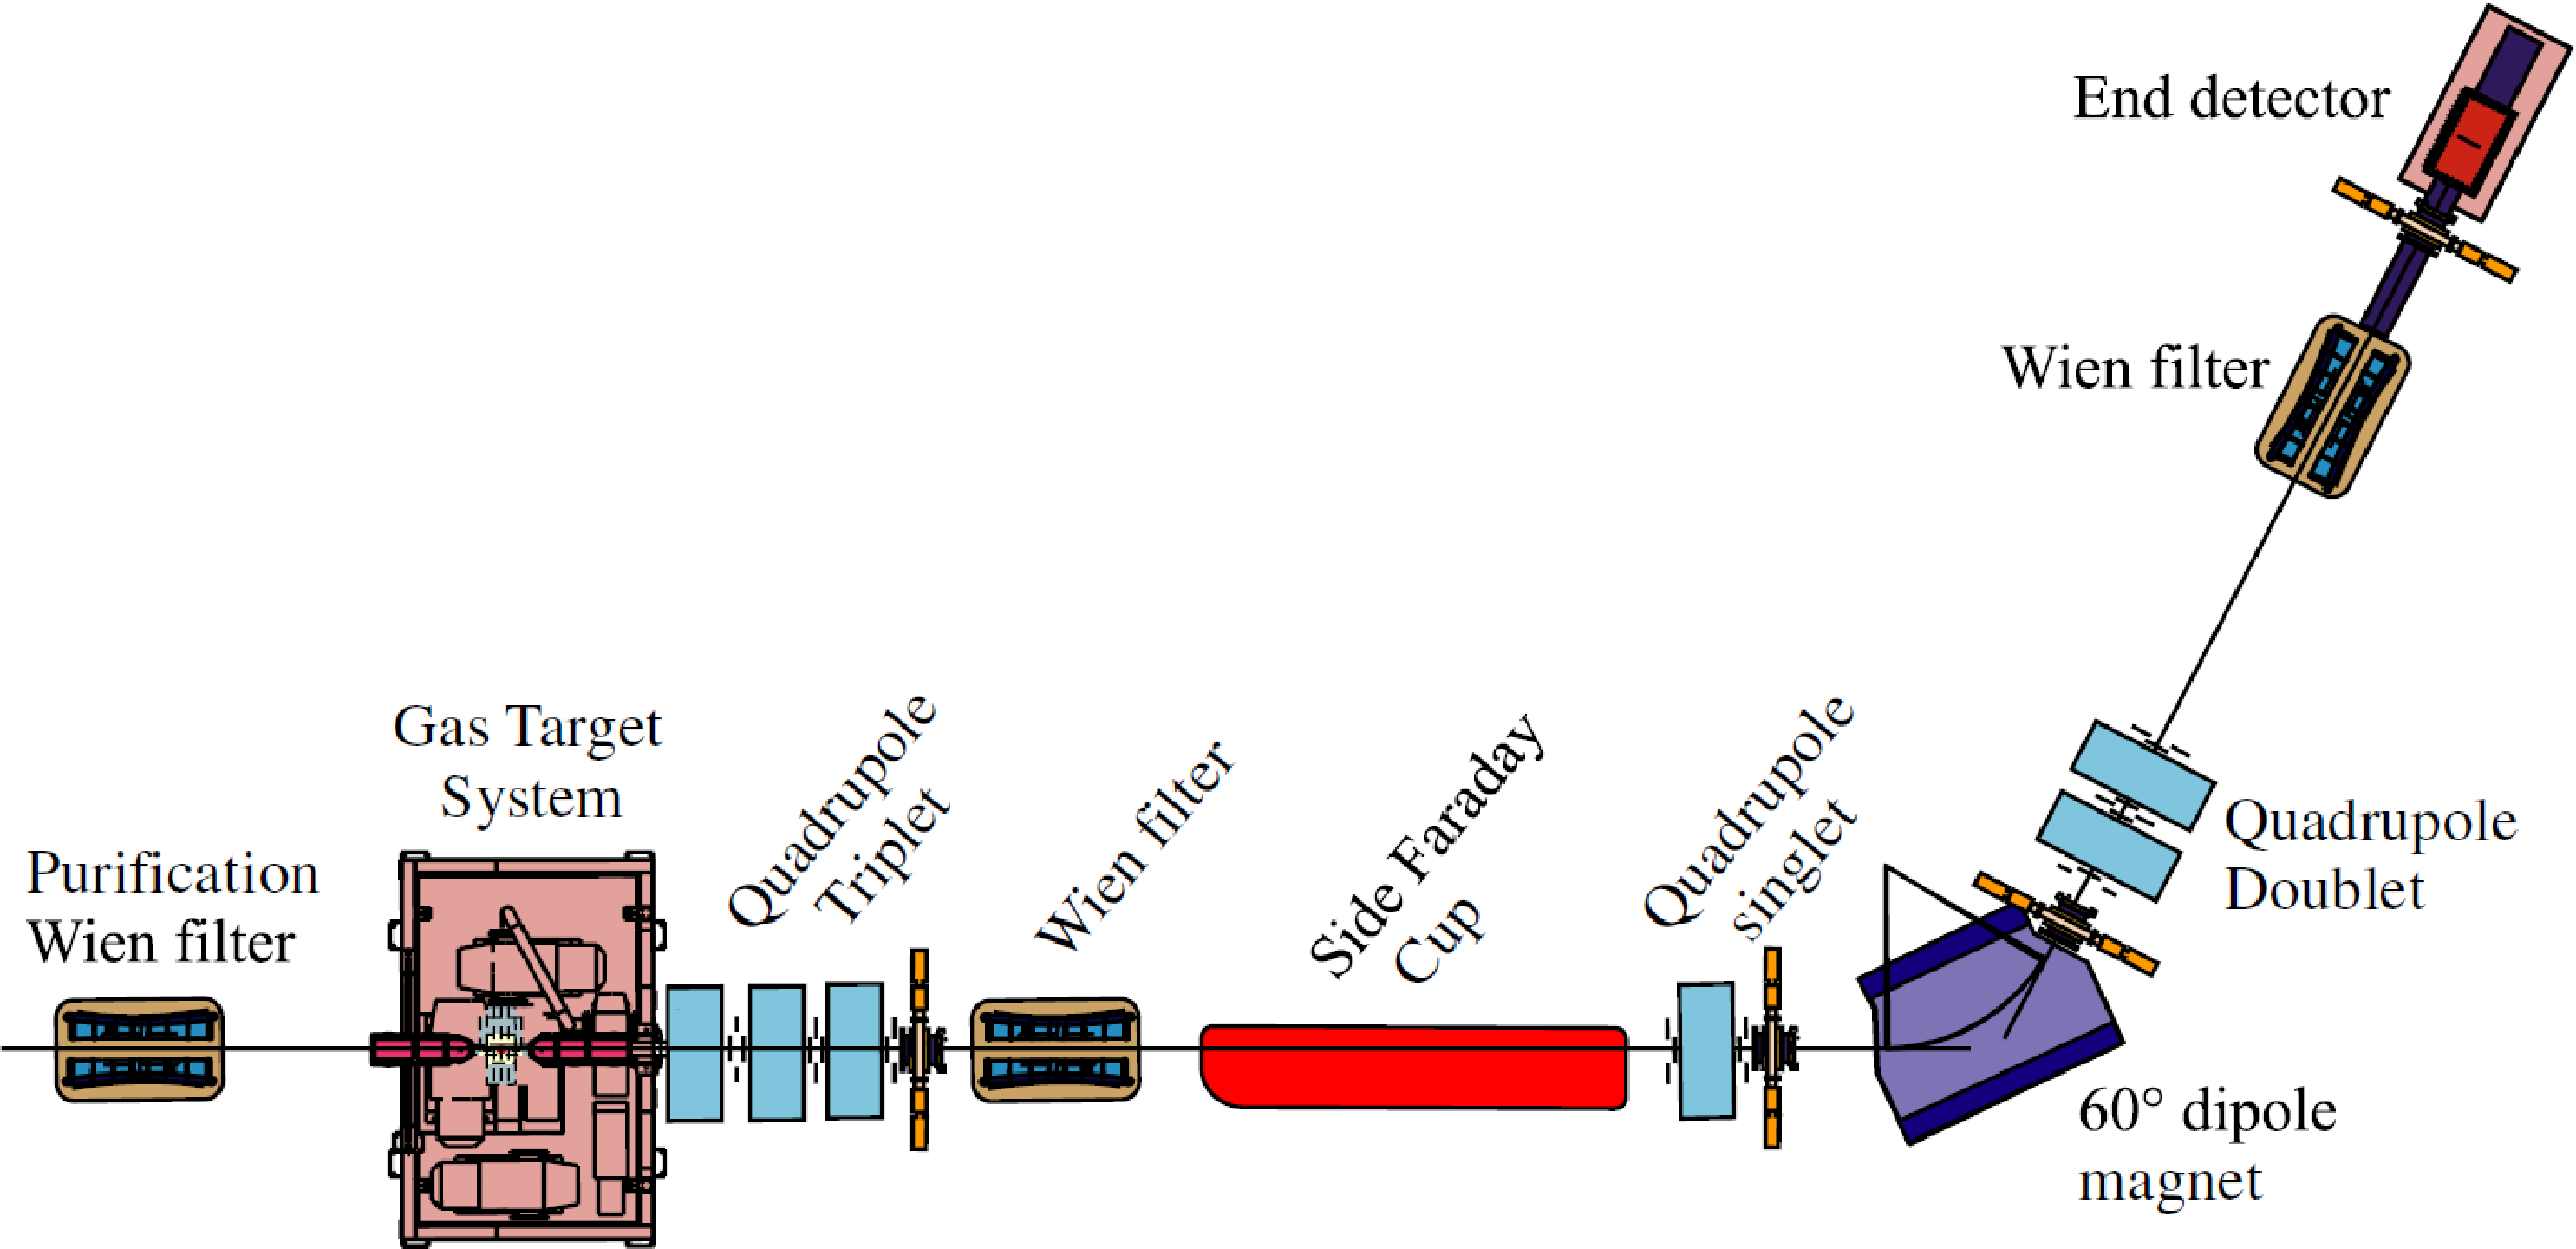
\includegraphics{DiLeva08_Fig2_ERNAschematic}
}
%\vspace{5cm}       % Give the correct figure height in cm
\caption{Schematic view of the ERNA recoil separator. Taken from \cite{dile08}.}
\label{fig:erna}       % Give a unique label
\end{figure}
Figure \ref{fig:erna} shows the eventual setup which in its design was limited by space considerations. For this reason the charge state selection follows the first velocity filter and not vice versa as in the NABONA experiment. The magnetic dipole is then followed by another crossed field (Wien-) filter device to increase beam suppression. The windowless gas target was constructed to allow placement of $\gamma$ detectors around the gas cell for $\gamma$-recoil coincidence measurements. Recoil detection was initially performed by a segmented ionization chamber but later replaced with a Time-of-flight-Energy (Tof-E) system consisting of a micro-channel plate mirror setup (Tof in conjunction with $\gamma$ detection) and a silicon strip detector. The performance parameters of the system were carefully explored in a series of measurements which are documented in several publications (\cite{roga99,roga03,gial04,schu04,dile08}) over a period of 10 years. ERNA was built for low energy measurements of the \nuc{12}{C}\reac{\alpha}{\gamma}\nuc{16}{O} reaction in inverse kinematics. Among the reactions targeted for proton and alpha radiative capture, this one is unfortunately the most demanding regarding required separator acceptance and beam suppression. The lowest energy in the centre-of-mass system where a measurement with currently available carbon ion beams of ten's of micro-Ampere seems feasible is about \EcmM{0.7}. Here, a separator needs to accept recoils with a half-angle of $q = 31 \unit{mrad}$ and $\frac{\Delta{}E}{E} = 12.8\%$. The requirements relax somewhat at higher energies to, {\it e.g.} \EcmM{5}: $q = 18 \unit{mrad}$ and $\frac{\Delta{}E}{E} = 7.2\%$. ERNA was nearly able to achieve the low energy benchmark but at the cost of lower beam suppression ranging between $10^{-10}$ and $10^{-12}$ dependent on recoil energies (better at higher energies). An interesting point to note is that the beam suppression deteriorated by a factor of 20 when gas was present in the cell compared to a run without gas. The reason could be additional energy and angle straggling, but most likely is due to the fact that a range of charge states is produced, which in the ERNA design does not filter out in the first selection stage, and which through additional scattering can reach the final focal plane. The tests of the segmented ionization chamber combined with the beam suppression available from the separator revealed that its performance was not sufficient to cover the full targeted energy range for the \nuc{12}{C}\reac{\alpha}{\gamma}\nuc{16}{O} reaction, as the ``leaky'' beam signature encroached on the \nuc{16}{O} recoil signal already at centre-of-mass energies of 2 MeV. An estimate was given that with the available setup measurements down to approximately \EcmM{1.3} would be possible. Improved recoil identification was later provided by adding in the $\gamma$-MCP detector Tof-E condition. As this review focusses on the results of radiative capture measurements using recoil separators with radioactive ion beams, we refer the reader for ERNA scientific results to \cite{schu05} (\nuc{12}{C}\reac{\alpha}{\gamma}\nuc{16}{O}) and \cite{dile09} (\nuc{3}{He}\reac{\alpha}{\gamma}\nuc{7}{Be}).
